\documentclass[Madrid]{beamer}
\usepackage{graphicx,url}
\usepackage{float}
\usepackage[brazil]{babel}   
\usepackage[utf8]{inputenc}
\usepackage{amsmath}
\begin{document}

\author{Christian Nakata, Kevin Levrone, Pedro Rocha e Rafael Sanchez}
\title{Inteligência Artificial II - Primeiro Trabalho}
\maketitle

\begin{frame}
	\frametitle{Resumo}
	Esse trabalho propõe a confecção de um modelo de rede de crença para realizar predições na bolsa de valores BOVESPA. Com base nesse modelo, uma implementação foi realizada em Python para analisar dados históricos de 11 empresas diferentes, parametrizando o modelo de predição com esses dados. Esse programa é capaz de prever a melhor empresa para se investir no próximo dia, com base em informações sobre os 5 dias úteis anteriores.  
\end{frame}

\begin{frame}
	\frametitle{Redes de Crença}
	Abordagem teórica breve sobre redes de crença
\end{frame}

\begin{frame}
	\frametitle{Modelo Desenvolvido}
	
	Para a rede Bayesiana proposta, definiu-se uma variável aleatória trivalente para indicar o comportamento do preço de uma ação $x$ na transição de um dia \textbf{$A_i$} para o próximo dia útil \textbf{$A_{i+1}$}. Ela é definida da seguinte forma:
	
\begin{equation}
	S_x(A_i, A_{i+1}) = \begin{cases}	\text{desvalorizou} & \text{, se } v < -5\%\\
								\text{permaneceu} & \text{, se } -5\% \leq v \leq +5\%\\
								\text{valorizou} & \text{, se } v > +5\%\end{cases}
\end{equation}

	No qual $v$ é a variação percentual do preço da ação $x$.
\end{frame}

\begin{frame}
	\frametitle{Modelo Desenvolvido}
	
	Considerando a variação de preço para papéis de $n$ empresas $x_1, x_2 ... x_n$ em 3 dias consecutivos ($A_1$, $A_2$ e $A_3$), tem-se a seguinte rede Bayesiana:
	
	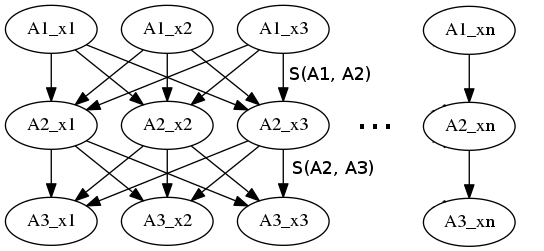
\includegraphics[scale=0.5]{bayes.png}
\end{frame}

\begin{frame}
	\frametitle{Modelo Desenvolvido}
	
	\begin{itemize}
		\item O objetivo é estimar qual ação $x_i$ tem a maior probabilidade de fechar em alta no terceiro dia, dados os valores de fechamento do pregão para os dois dias anteriores.
		\item Umas vez que as empresas $x_i$ escolhidas são todas do mesmo setor (tecnologia), optou-se por estabelecer relações de dependência entre suas variações.
	\end{itemize}
\end{frame}

\begin{frame}
	\frametitle{Probabilidades a se definir}
	Analisando os dados históricos, deve-se definir, portanto, as probabilidades:
	
	\begin{equation}
		P(S_{x_i}(A2, A3) | S_{x_1}(A1, A2), S_{x_2}(A1, A2) ... S_{x_n}(A1, A2) 
	\end{equation}
	
	para cada empresa $x_i$ indicada no estudo. Essas probabilidades permitem estimar se as ações fecharão o próximo dia valorizadas, desvalorizadas ou sem alteração de preço. 
\end{frame}

\end{document}